\chapter{実験と結果}	% TODO: 章題を記入.題は任意.
\thispagestyle{plain}   % chapterの直後に必ず指定

%TODO: 章の内容を記入.以下はサンプル.
\section{ビルドモードでの構造物生成の実験}\label{sec:build_mode_generate}
\ref{sec:build_mode}節にて解説したビルドモードについて,①``station''や②``japanese castle''とプロンプトを与えた際の生成結果を図\ref{fig:station1},図\ref{fig:j_castle1}に示す.
\begin{figure}[H]
    \centering
    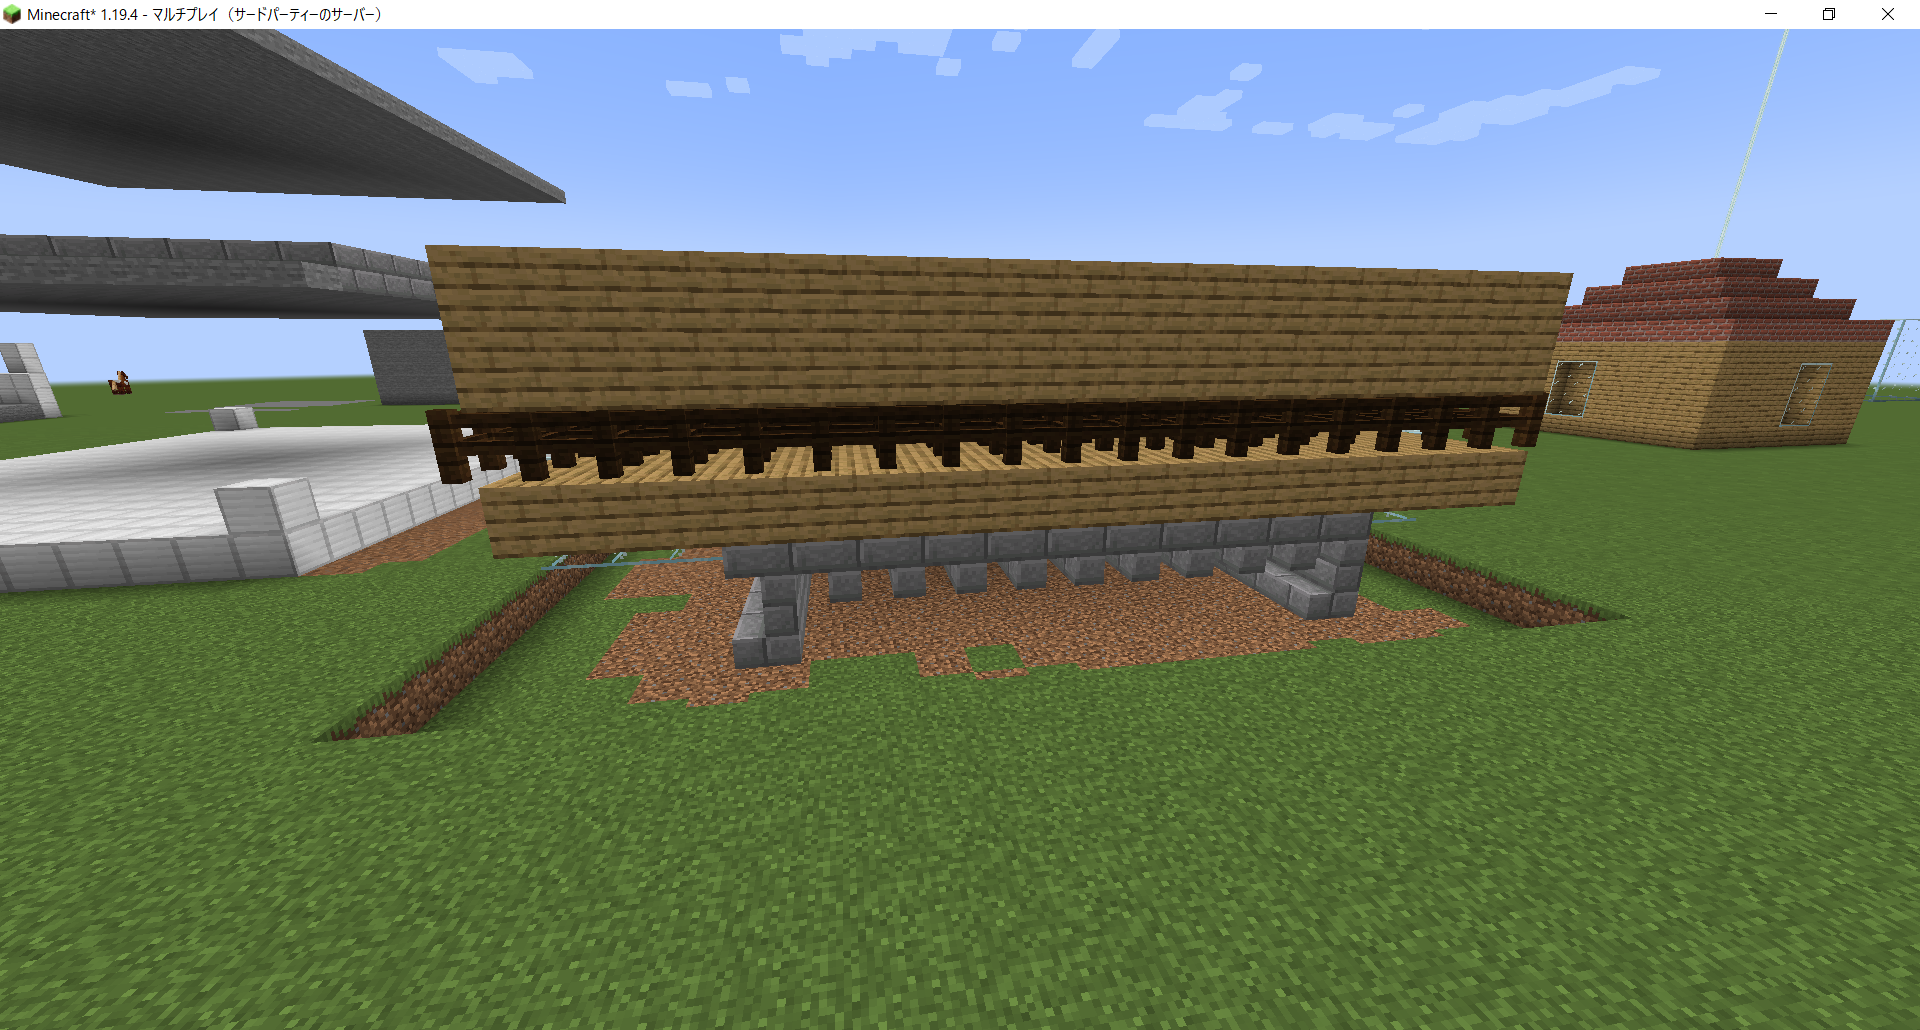
\includegraphics[width=0.8\textwidth]{fig/station1.png}
    \caption{①の生成結果}
    \label{fig:station1}
\end{figure}

\begin{figure}[H]
    \centering
    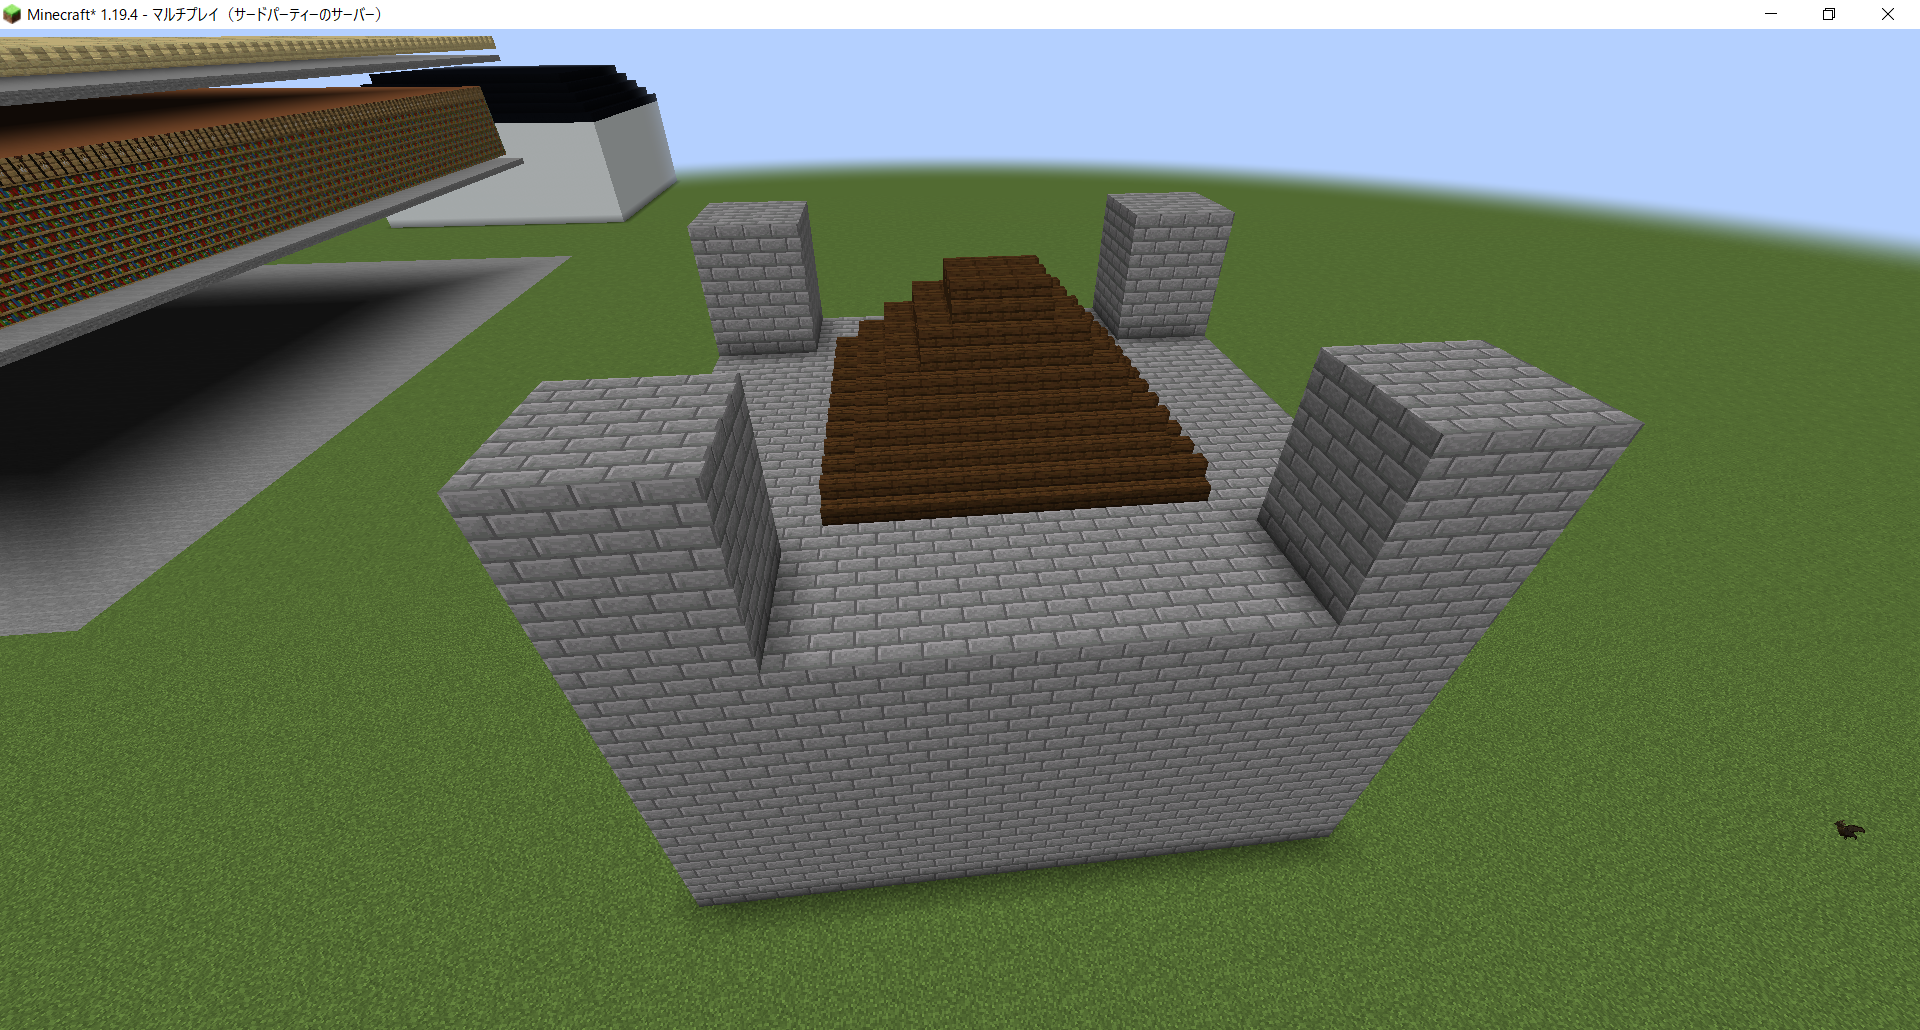
\includegraphics[width=0.8\textwidth]{fig/j_castle1.png}
    \caption{②の生成結果}
    \label{fig:j_castle1}
\end{figure}

生成結果を見ると,図\ref{fig:station1}では駅のような外観は出来ているものの,駅の特徴を表すレールなどのブロックが置かれていないことが分かる.
また,図\ref{fig:j_castle1}では,砦や城のような構造物ではあるものの,日本風ではないことが分かる.

これらの生成結果を改善するために③``Build a train station. I want the tracks to use rails. And build the platform well.'',④``Build a Japanese castle. Since it is a Japanese castle, the walls are white and the roof is black. The floor size should get smaller as you go higher up. Please make about 5 floors. Also, please make a stone wall.''のプロンプトを与えた.生成結果を図\ref{fig:station2},図\ref{fig:j_castle2}に示す.

\begin{figure}[H]
    \centering
    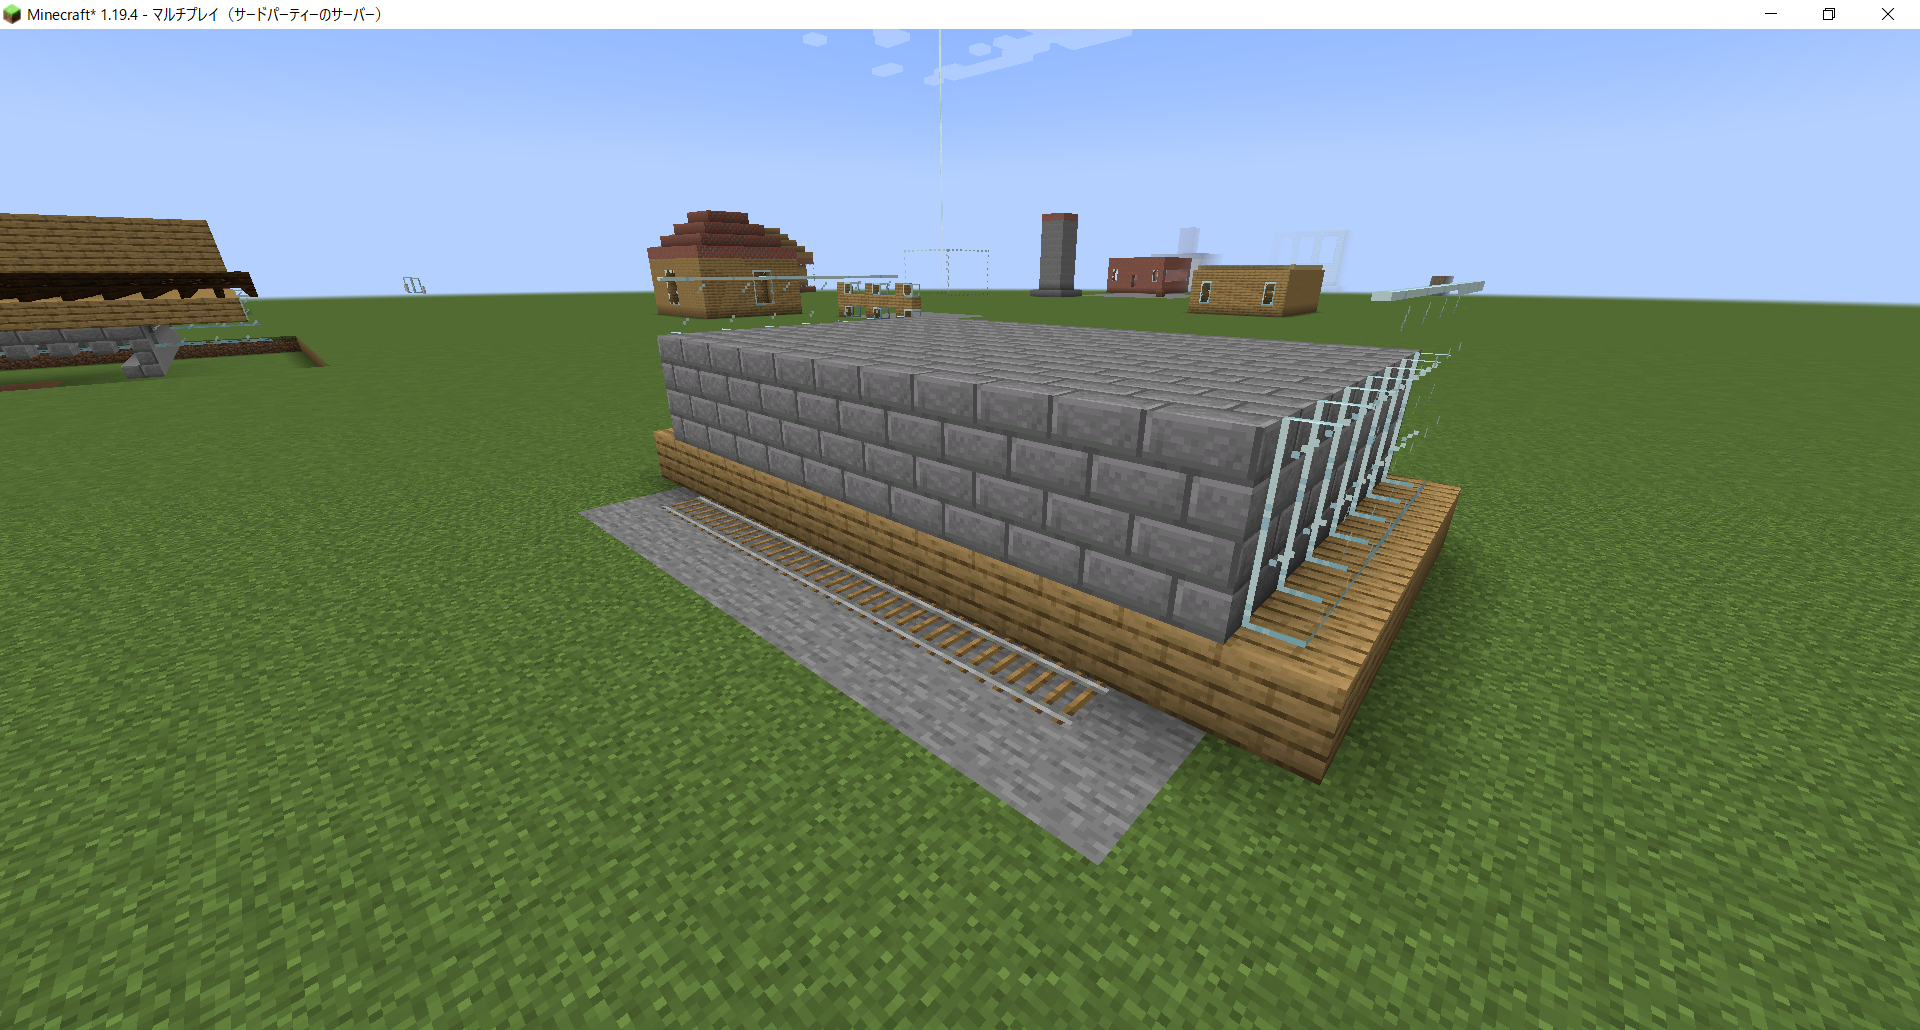
\includegraphics[width=0.8\textwidth]{fig/station2.png}
    \caption{③の生成結果}
    \label{fig:station2}
\end{figure}

\begin{figure}[H]
    \centering
    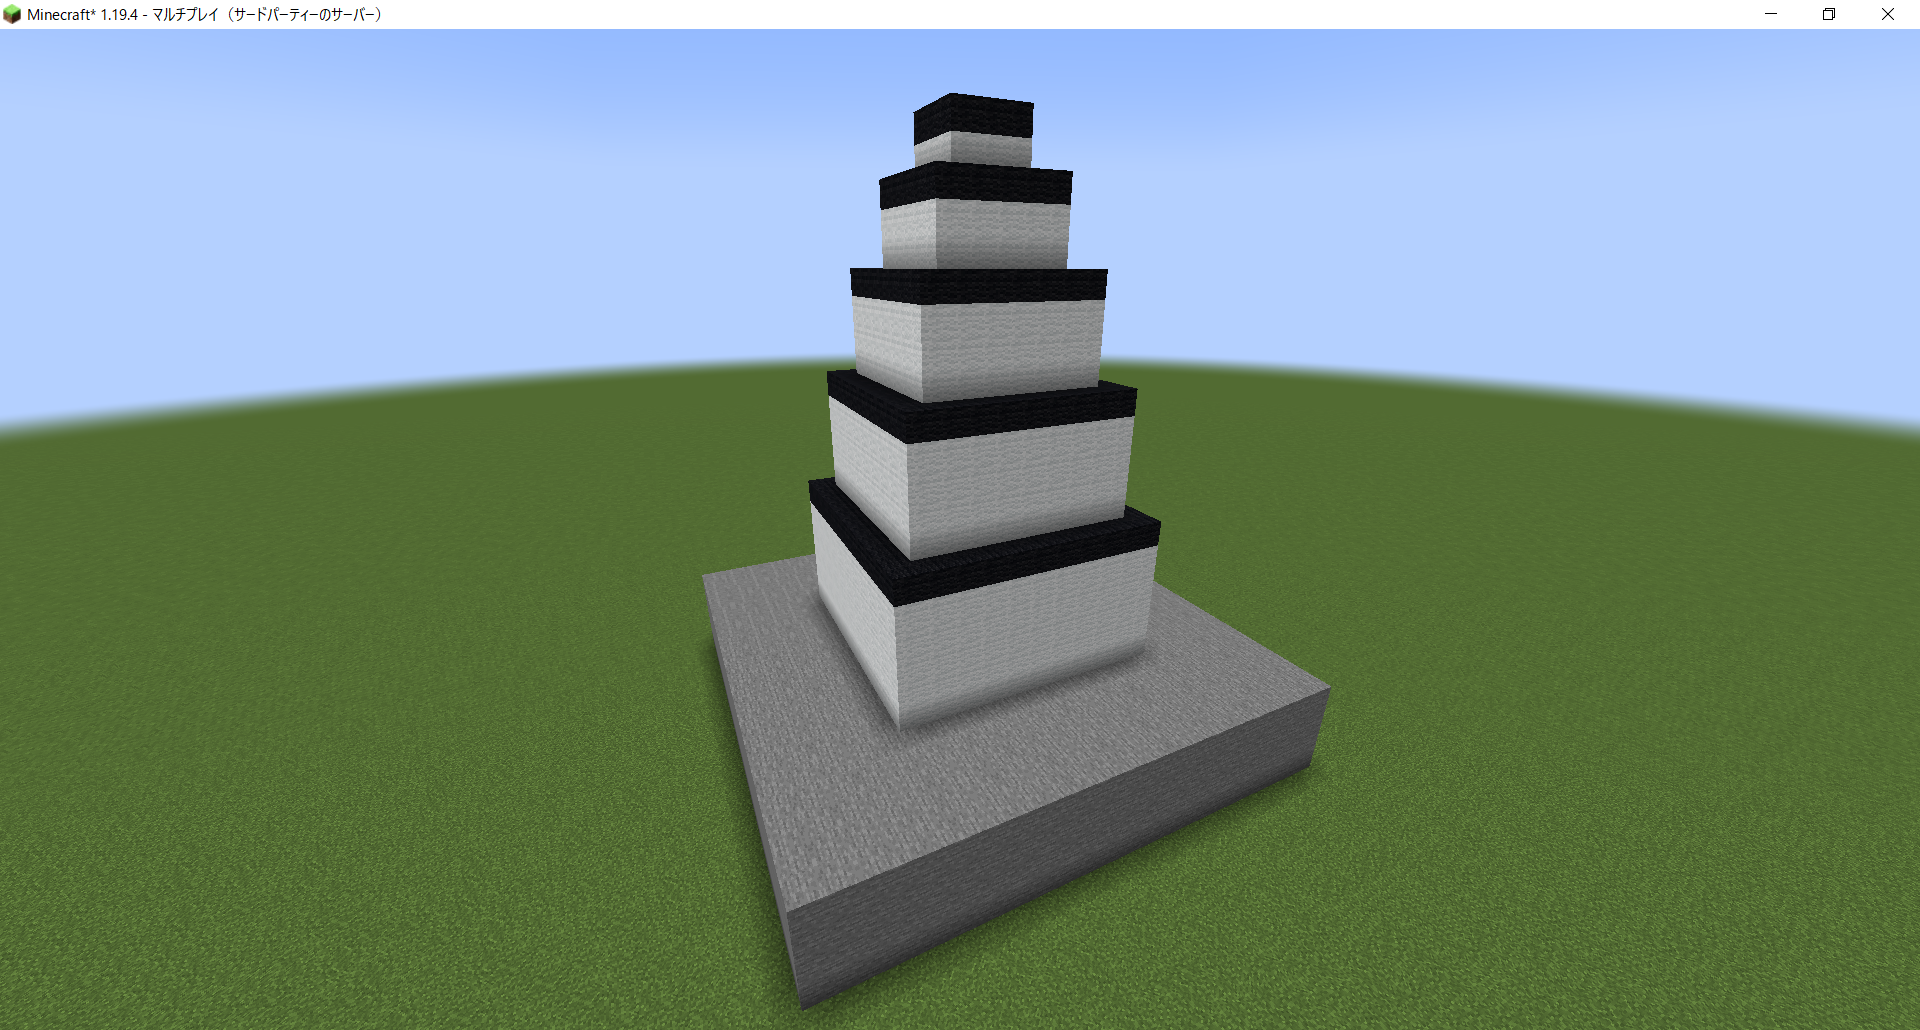
\includegraphics[width=0.8\textwidth]{fig/j_castle2.png}
    \caption{④の生成結果}
    \label{fig:j_castle2}
\end{figure}

生成結果を見ると,図\ref{fig:station2}はプラットフォームに沿ってレールが敷かれており,図\ref{fig:j_castle2}では細部は出来ていないものの日本風の城の形が出来ていることから,結果が改善されたことが分かる.

このようにLLMが仮想的な3D世界で構造物を作る例はほとんど存在せず,プロンプトエンジニアリングを駆使して自身の想像した構造物を形成することの最初の段階として,興味深い結果を示している.

\section{アンケート}
BOTの有用性を検証するためBOTのデモとアンケートを実施した.
デモ・アンケートは2023年10月16日に開催された,公立はこだて未来大学オープンラボの,イアンフランク研ブースにて行われ,計16人の学生がデモを行いアンケートに回答した.
デモではBOTとの会話を始めに体験していただき,その後,ビルドモードを体験するように促した.

\section{アンケートの結果・考察}
デモを行った後のアンケートの結果の一例について表\ref{tab:answer1},表\ref{tab:answer2}に示す.

``このBOTを使うことで新しい建築のアイデアやインスピレーションを得ることができましたか?''という質問について,``そう思う''を4,``どちらかというとそう思う''を3,``どちらかというとそう思わない''を2,``そう思わない''を1として平均を計算した結果,3.2 となった.
また,``このBOTを使うことでLLM(ChatGPTなど)の使い方を新しく学ぶことができましたか?''の質問については同様の方法で平均を求めた結果,3.47となった.

そう思う~そう思わないの4段階の同じ指標で回答してもらった結果,表\ref{tab:answer2}の結果のみ平均3.47と高かったことから,BOTによってLLMの新しい使い方を学べたことが示唆された.
表\ref{tab:answer1}の結果では肯定的な意見が得られているものの,表\ref{tab:answer2}の結果より平均が低いことや\ref{sec:build_mode_generate}節の生成結果から考察するとビルドモードは改善の必要があると考えられる.
\begin{table}[H]
    \centering
    \caption{このBOTを使うことで新しい建築のアイデアやインスピレーションを得ることができましたか?}
    \label{tab:answer1}
    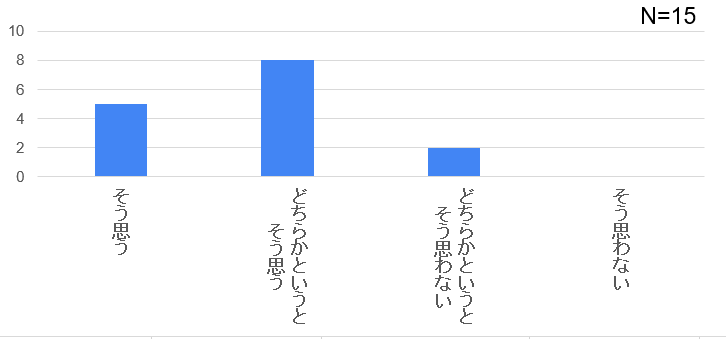
\includegraphics[width=0.8\textwidth]{fig/tab2.png}
\end{table}

\begin{table}[H]
    \centering
    \caption{このBOTを使うことでLLM(ChatGPTなど)の使い方を新しく学ぶことができましたか?}
    \label{tab:answer2}
    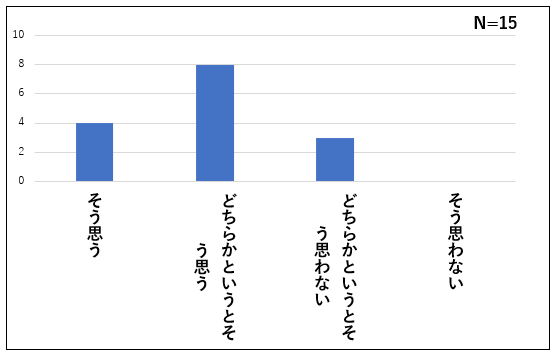
\includegraphics[width=0.8\textwidth]{fig/tab3.png}
\end{table}


